\documentclass[tikz,border=15pt]{standalone}
\usepackage{tikz}
\usepackage{xcolor}
\usetikzlibrary{arrows.meta,calc,positioning,shapes.geometric}

\definecolor{bgcolor}{RGB}{11,15,25}
\definecolor{cardbg}{RGB}{30,41,59}
\definecolor{cardborder}{RGB}{51,65,85}
\definecolor{goldborder}{RGB}{251,191,36}
\definecolor{goldbg}{RGB}{69,26,3}
\definecolor{goldbadge}{RGB}{133,77,14}
\definecolor{goldtext}{RGB}{254,243,199}
\definecolor{blueborder}{RGB}{56,189,248}
\definecolor{bluebg}{RGB}{23,37,84}
\definecolor{bluebadge}{RGB}{3,105,161}
\definecolor{bluetext}{RGB}{125,211,252}
\definecolor{greenborder}{RGB}{52,211,153}
\definecolor{greenbg}{RGB}{6,78,59}
\definecolor{greentext}{RGB}{167,243,208}
\definecolor{vdbdark}{RGB}{2,44,34}
\definecolor{purpleborder}{RGB}{192,132,252}
\definecolor{purplebg}{RGB}{76,29,149}
\definecolor{purpletext}{RGB}{243,232,255}
\definecolor{promptdark}{RGB}{46,16,101}
\definecolor{slategray}{RGB}{148,163,184}

\begin{document}
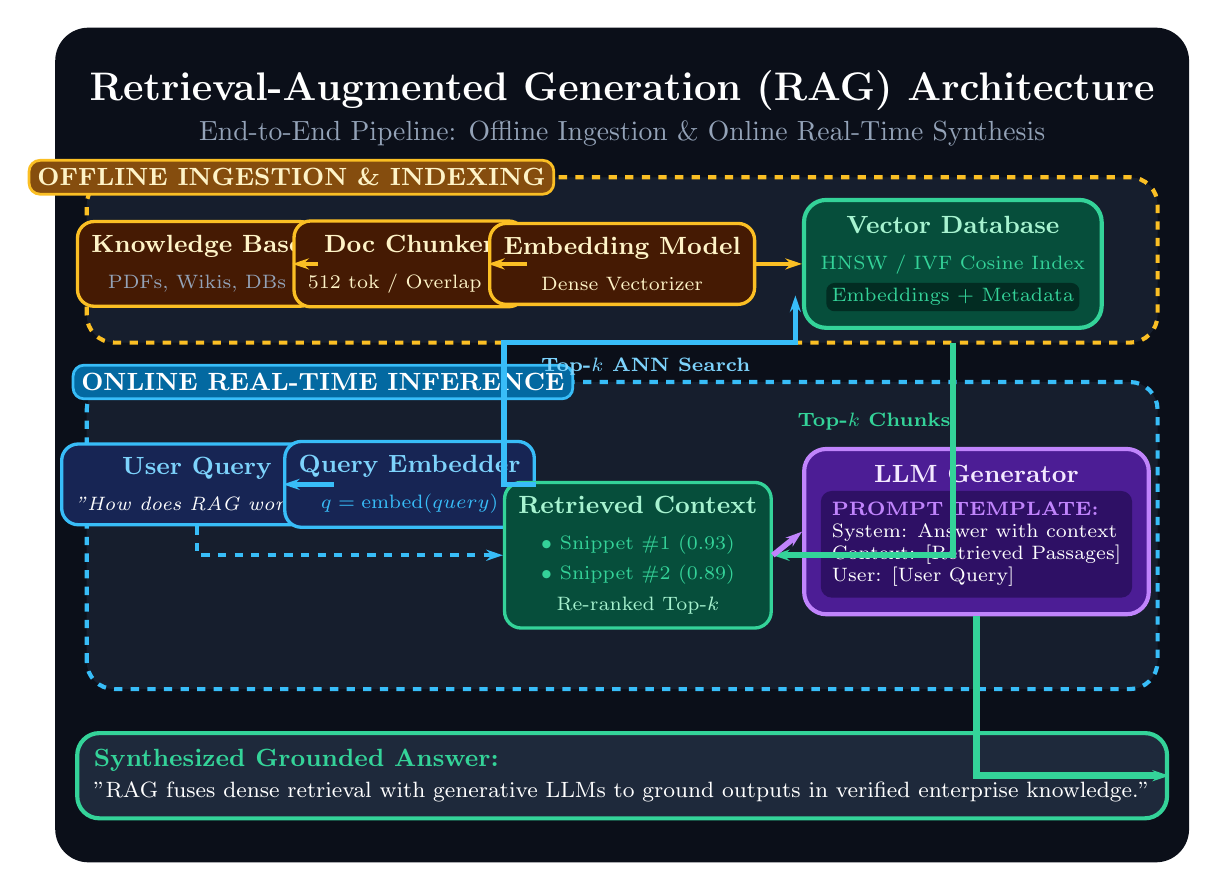
\begin{tikzpicture}[
    >={Stealth[length=6pt, width=4pt]}
]

% Background Card
\fill[rounded corners=12pt, fill=bgcolor] (-7.2,-5.4) rectangle (7.2,5.2);

% Title & Header
\node[text=white, font=\Large\bfseries] at (0, 4.4) {Retrieval-Augmented Generation (RAG) Architecture};
\node[text=slategray, font=\normalsize] at (0, 3.85) {End-to-End Pipeline: Offline Ingestion \& Online Real-Time Synthesis};

% 1. OFFLINE INGESTION PIPELINE (Top Box)
\draw[goldborder, dashed, line width=1.5pt, fill=cardbg, fill opacity=0.6, rounded corners=10pt] (-6.8, 1.2) rectangle (6.8, 3.3);
\node[fill=goldbadge, draw=goldborder, line width=1pt, rounded corners=4pt, text=goldtext, font=\small\bfseries, inner sep=3pt] at (-4.2, 3.3) {OFFLINE INGESTION \& INDEXING};

% Offline Nodes
% Docs
\node[fill=goldbg, draw=goldborder, line width=1.2pt, rounded corners=6pt, text=white, font=\small, align=center, inner sep=5pt] (DOCS) at (-5.4, 2.2) {
    \textbf{\textcolor{goldtext}{Knowledge Base}}\\[2pt]
    \textcolor{slategray}{\scriptsize PDFs, Wikis, DBs}
};

% Chunker
\node[fill=goldbg, draw=goldborder, line width=1.2pt, rounded corners=6pt, text=white, font=\small, align=center, inner sep=5pt] (CHUNK) at (-2.7, 2.2) {
    \textbf{\textcolor{goldtext}{Doc Chunker}}\\[2pt]
    \textcolor{goldtext}{\scriptsize 512 tok / Overlap 50}
};

% Embedder (Offline)
\node[fill=goldbg, draw=goldborder, line width=1.2pt, rounded corners=6pt, text=white, font=\small, align=center, inner sep=5pt] (OFF_EMB) at (0.0, 2.2) {
    \textbf{\textcolor{goldtext}{Embedding Model}}\\[2pt]
    \textcolor{goldtext}{\scriptsize Dense Vectorizer}
};

% Vector DB (Top Right)
\node[fill=greenbg, draw=greenborder, line width=1.5pt, rounded corners=8pt, text=white, font=\small, align=center, inner sep=6pt] (VDB) at (4.2, 2.2) {
    \textbf{\textcolor{greentext}{Vector Database}}\\[2pt]
    \textcolor{greenborder}{\scriptsize HNSW / IVF Cosine Index}\\[2pt]
    \tikz \node[fill=vdbdark, rounded corners=3pt, text=greenborder, font=\scriptsize, inner sep=2pt] {Embeddings + Metadata};
};

% Ingestion Arrows
\draw[goldborder, line width=1.5pt, ->] (DOCS) -- (CHUNK);
\draw[goldborder, line width=1.5pt, ->] (CHUNK) -- (OFF_EMB);
\draw[goldborder, line width=1.5pt, ->] (OFF_EMB) -- (VDB);

% 2. ONLINE INFERENCE PIPELINE (Middle Box)
\draw[blueborder, dashed, line width=1.5pt, fill=cardbg, fill opacity=0.6, rounded corners=10pt] (-6.8, -3.2) rectangle (6.8, 0.7);
\node[fill=bluebadge, draw=blueborder, line width=1pt, rounded corners=4pt, text=white, font=\small\bfseries, inner sep=3pt] at (-3.8, 0.7) {ONLINE REAL-TIME INFERENCE};

% User Query
\node[fill=bluebg, draw=blueborder, line width=1.2pt, rounded corners=6pt, text=white, font=\small, align=center, inner sep=5pt] (QUERY) at (-5.4, -0.6) {
    \textbf{\textcolor{bluetext}{User Query}}\\[2pt]
    \textcolor{white}{\itshape\scriptsize "How does RAG work?"}
};

% Query Embedder
\node[fill=bluebg, draw=blueborder, line width=1.2pt, rounded corners=6pt, text=white, font=\small, align=center, inner sep=5pt] (Q_EMB) at (-2.7, -0.6) {
    \textbf{\textcolor{bluetext}{Query Embedder}}\\[2pt]
    \textcolor{blueborder}{\scriptsize $q = \mathrm{embed}(query)$}
};

% Retrieved Context Box
\node[fill=greenbg, draw=greenborder, line width=1.2pt, rounded corners=6pt, text=white, font=\small, align=center, inner sep=5pt] (CONTEXT) at (0.2, -1.5) {
    \textbf{\textcolor{greentext}{Retrieved Context}}\\[2pt]
    \textcolor{greenborder}{\scriptsize $\bullet$ Snippet \#1 (0.93)}\\
    \textcolor{greenborder}{\scriptsize $\bullet$ Snippet \#2 (0.89)}\\
    \textcolor{greentext}{\scriptsize Re-ranked Top-$k$}
};

% LLM Generator Box
\node[fill=purplebg, draw=purpleborder, line width=1.5pt, rounded corners=8pt, text=white, font=\small, align=center, inner sep=6pt] (LLM) at (4.5, -1.2) {
    \textbf{\textcolor{purpletext}{LLM Generator}}\\[2pt]
    \tikz \node[fill=promptdark, rounded corners=4pt, text=white, font=\scriptsize, align=left, inner sep=4pt] {
        \textcolor{purpleborder}{\bfseries PROMPT TEMPLATE:}\\
        System: Answer with context\\
        Context: [Retrieved Passages]\\
        User: [User Query]
    };
};

% Online Flow Arrows
\draw[blueborder, line width=2pt, ->] (QUERY) -- (Q_EMB);

% Query Search to Vector DB
\draw[blueborder, line width=2pt, ->] (Q_EMB.east) -- (-1.5, -0.6) -- (-1.5, 1.2) -- (2.2, 1.2) -- (2.2, 1.8);
\node[text=bluetext, font=\scriptsize\bfseries] at (0.3, 0.9) {Top-$k$ ANN Search};

% Vector DB return to Context
\draw[greenborder, line width=2pt, ->] (4.2, 1.2) |- (CONTEXT.east);
\node[text=greenborder, font=\scriptsize\bfseries] at (3.2, 0.2) {Top-$k$ Chunks};

% Direct Query augmentation path
\draw[blueborder, dashed, line width=1.5pt, ->] (QUERY.south) |- (CONTEXT.west);

% Context to LLM
\draw[purpleborder, line width=2pt, ->] (CONTEXT.east) -- (LLM.west);

% 3. FINAL SYNTHESIZED ANSWER (Bottom Box)
\node[fill=cardbg, draw=greenborder, line width=1.5pt, rounded corners=8pt, text=white, font=\small, align=left, inner sep=6pt] (ANSWER) at (0, -4.3) {
    \textbf{\textcolor{greenborder}{Synthesized Grounded Answer:}}\\
    \textcolor{white}{\footnotesize "RAG fuses dense retrieval with generative LLMs to ground outputs in verified enterprise knowledge."}
};
\draw[greenborder, line width=2.5pt, ->] (LLM.south) |- (ANSWER.east);

\end{tikzpicture}
\end{document}
